\chapter{Nuclear Uncertainties}
The theory covariance formalism developed in Chapter~\ref{chapter:thuncs} can be applied to any source of theory uncertainty in PDFs. One of the most important of these is nuclear uncertainties. A wide range of data is needed to pin down the form of PDFs, including that where the proton is not in a free state. More precisely, this encompasses DIS and DY fixed target measurements involving deuteron and heavy nuclear targets. In these cases the proton's interaction is altered due to the surrounding nuclear environment, and this difference propagates through to the fitted PDFs, leading to an unwanted shift in their central values and uncertainties. We cannot simply discard these data, as they play a crucial role in the strangeness content of the proton and also the light flavour separation at high $x$, a region important for searches for physics beyond the Standard Model. Instead, we must determine corrections to the PDF central value and additional uncertainties to account for the use of nuclear data.

Given their importance, there have been wide-ranging studies of deuteron and heavy nuclear corrections: deuteron corrections have been included in previous PDF determinations via nuclear smearing functions~\cite{Owens:2012bv,Ball:2013gsa,Harland-Lang:2014zoa,Accardi:2016qay,
  Alekhin:2017fpf} based on models of the deuteron wavefunction~\cite{Wiringa:1994wb,Melnitchouk:1994rv,Melnitchouk:1996vp,
  Machleidt:2000ge,Gross:2014wqa}; heavy nuclear corrections have been included following a selection of nuclear models~\cite{Harland-Lang:2014zoa,Dulat:2015mca,Alekhin:2017kpj} or fitting the data~\cite{Accardi:2016qay}. Using such models, however, can introduce a bias that is difficult to quantify. In the past, NNPDF has opted to ignore nuclear effects on the assumption that they are small~\cite{Ball:2013gsa, Ball:2014uwa, Ball:2017nwa}, however this is another source of uncertainty that is becoming increasingly important as PDF precision increases. Furthermore it is thought that the shape of PDFs can be affected, especially at high $x$~\cite{Owens:2012bv}, and this was evidenced in previous NNPDF fits with deuteron corrections following Eq.~(8) of~\cite{Harland-Lang:2014zoa}, with parameter values
from~\cite{Martin:2012da}; however, an increase in $\chi^2$ here suggested that the nuclear uncertainty was not effectively determined.
  
In this Chapter we show how to account for nuclear effects, both deuteron and heavy nuclear, in proton PDF fits. We do this using a theory covariance matrix of nuclear uncertainties, and propose two alternatives for their inclusion: one is to simply apply a nuclear uncertainty, effectively deweighting the affected datasets in the PDF fit proportionally; the other is to shift the PDF central values by applying a nuclear correction, applying smaller nuclear uncertainties as a result. If the shift is estimated accurately, then for an uncertainty smaller than the shift the second method gives a more precise outcome.

We can determine nuclear corrections by comparing the theory predictions for nuclear observables using proton PDFs with those using the correct nuclear PDF (nPDF). This shift can be identified with Eqn~\ref{eqn:thshift} in Chapter~\ref{chapter:thuncs}, i.e. quantifying the size of nuclear correction for that data point. The collective shifts can then be used to construct a theory covariance matrix based on Eqn~\ref{eqn:covmat_format_def}. In carrying out this work we looked first at heavy nuclear corrections (for Cu, Fe and Pb) and then at deuteron corrections, addressing them separately because deuterons, being only a proton and a neutron, are distinct from a heavy nuclear environment such as $^{56}$Fe, with 26 protons and 30 neutrons bound together. 

For the heavy nuclear PDFs we initially used~\cite{Ball:2018twp} a combination of three available nPDF sets (DSSZ~\cite{deFlorian:2011fp},
nCTEQ15~\cite{Kovarik:2015cma}, and EPPS16~\cite{Eskola:2016oht}), but NNPDF subsequently released its own global nPDFs, nNNPDF2.0~\cite{AbdulKhalek:2020yuc}, which is what we will consider in this Chapter. Given the enhanced difficulty of nPDF determination, all of these nPDF sets are only available at NLO. For the deuteron PDFs we developed a self-consistent iterative procedure to determine deuteron PDFs at NNLO within the NNPDF formalism, and used the output of this to determine deuteron corrections. These deuteron PDFs have the advantage over those from nNNPDF2.0 that they are NNLO, but are based on less data so have larger uncertainties. This should at worst lead to a conservative uncertainty estimation, but we will discuss the comparison in Section~\ref{sec:summandoutlook}.

This chapter is organised as follows. First we review the nuclear data in proton PDF fits (Sec.~\ref{sec:nucdat}). Then we consider heavy nuclear uncertainties including the resulting covariance matrix. We then look at deuteron uncertainties in the same way (Sec.~\ref{sec:deutunc}), before  including combined nuclear uncertainties in NNPDF4.0 proton PDF fits in Sec~\ref{sec:nucpdfs}. We summarise the results in Sec.~\ref{sec:summandoutlook}.

\section{Nuclear data in PDFs}
\label{sec:nucdat}
We consider the NNPDF3.1 NNLO dataset which consists of $\sim$ 4000 data points, of which $\sim$ 10\% is deuteron data and $\sim$ 20\% is heavy nuclear data. The table below summarises the datasets which make up the total nuclear data, giving the name of dataset, the observable it corresponds to, and the nuclear target involved.
\begin{center}
%\rowcolors{3}{blue!40!}{blue!20!}
\begin{tabular}{ |p{4cm}|p{7cm}|p{2cm}|  }
\hline
\multicolumn{3}{|c|}{Nuclear data} \\
\hline
Dataset & Observable & Target \\
\hline
\rowcolor{blue!20}
SLAC~\cite{Whitlow:1991uw}& DIS structure functions $F_2^d$ & Deuterium  \\
\rowcolor{blue!20}
BCDMS~\cite{Benvenuti:1989fm} & DIS structure functions $F_2^d$ & Deuterium \\
\rowcolor{blue!20}
NMC~\cite{Arneodo:1996kd} & DIS structure function ratios $F_2^d/F_2^p$ & Deuterium \\
\rowcolor{blue!20}
DYE866/NuSea~\cite{Towell:2001nh} & DY cross section ratios $\sigma^{\rm DY}_{pd}/\sigma^{\rm DY}_{pp}$ & Deuterium \\
\hline
\rowcolor{blue!40}
CHORUS~\cite{Onengut:2005kv} & CC DIS cross sections & $^{208}_{82}$Pb  \\
\rowcolor{blue!40}
NuTeV~\cite{Tzanov:2005kr} & DIS dimuon cross sections & $^{56}_{26}$Fe  \\
\rowcolor{blue!40}
DYE605~\cite{Heinrich:1989cp} & DY dimuon cross sections & $^{64}_{32}$Cu  \\
\hline
\end{tabular}
\end{center}
\section{Heavy nuclear uncertainties}
\label{sec:hnucunc}
Heavy nuclear uncertainties can be included using the covariance matrix methodology discussed in Chapter~\ref{chapter:thuncs}.
Each contribution to the covariance matrix, can be determined
\be 
\Delta_i^{(k)} = T_i^N[f_N^{(k)}] - T_i^N[f_p],
\ee 
where $T_i^N$ are the nuclear observables for the $i$-th data point, $f_N^{(k)}$ is a nuclear PDF replica indexed by $k$ and $f_p$ is the central value of the proton PDF. This is the difference between the obervable calculated with a given replica of the ``correct" nuclear PDF and the current value, which is calculated with the proton PDF. Including $N_{rep}$ contributions, one for each replica, $k$, means that the uncertainty in the nPDF is automatically incorporated into the nuclear uncertainty. A covariance matrix can then be constructed as
\be 
S_{ij} = \frac{1}{N_{rep}} \sum_k^{N_{rep}} \Delta_i^{(k)} \Delta_j^{(k)} .
\ee
A more ambitious approach is to also try and correct the value of the nuclear observable we use, so that it is based on the nPDF rather than the proton one. This can be done by applying a shift,
\be 
\delta T_i^N = T_i^N[f_N] - T_i^N [f_p],
\ee
to the nuclear observables. In this case we must amend the contributions to the covariance matrix so that they are
\be 
\Delta_i^{(k)} = T_i^N[f_N^{(k)}] - T_i^N[f_N].
\ee 
If the shift is accurate enough and greater than the uncertainty then this latter method should lead to a better fit. 

In the above equations the nuclear observables, $T_i^N$, are calculated from the proton observables, $T_i$, by taking into account the non-isoscalarity of the target, i.e. by combining the proton and neutron observables in accordance with the atomic number, $Z$ and mass number, $A$. Explicitly,
\be 
\begin{split}
T_i^N[f_p] &= \frac{1}{A} \bigg( Z T_i[f_p] + (A-Z) T_i[f_n] \bigg), \\
T_i^N[f_N] &= \frac{1}{A} \bigg( Z T_i[f_{p/N}] + (A-Z) T_i[f_{n/N}] \bigg).
\end{split}
\ee
The first line is what is done in standard NNPDF fits, and the second line is the extension to the nPDF case. Here $f_{p/N}$ is the PDF for the proton bound in a nucleus, $N$, and $f_{n/N}$ is the same for the neutron. We assume that the two are related by swapping $u$ and $d$ quarks. We obtain these PDFs directly from nNNPDF2.0, but they relate to $f_N$ via
\be 
f_N = \frac{1}{A} \bigg( Z f_{p/N} + (A-Z) f_{n/N} \bigg).
\ee
%%%%%%%%%%%%%%%%%%%%%%%%%%%%%%%%%%%%%%%%%%%%%%%%%%%%%%%%%%%%%%%%%%%%%
\begin{figure}[h]
  \begin{center}
    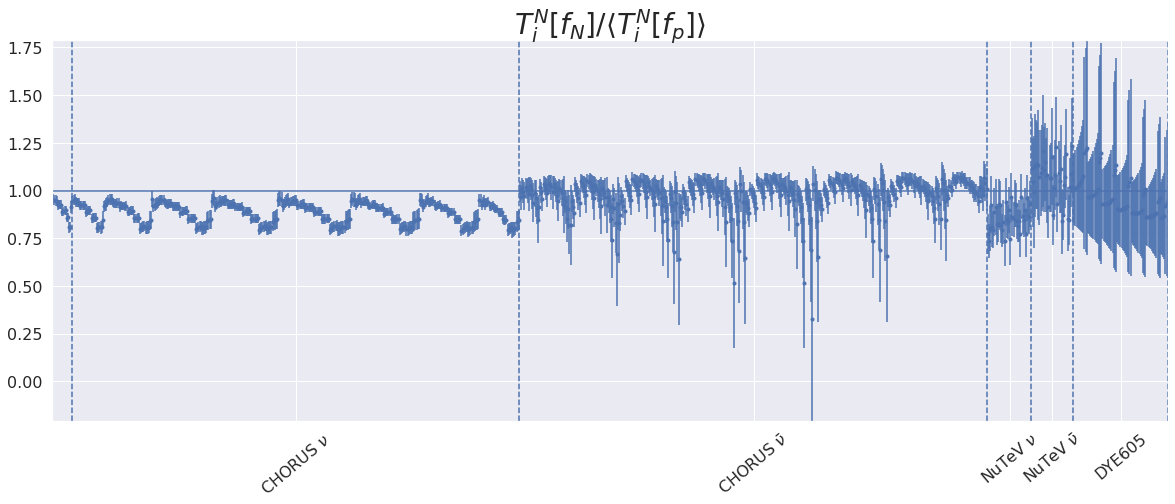
\includegraphics[width=\linewidth]{nuclear/plots/observable_ratio_nuclear.png}
   \caption{ Ratio between the nuclear observables computed with nPDFs, $T_i^N[f_N]$, and the central prediction computed with proton PDFs, $\langle T_i^N[f_p] \rangle$. The error is the standard deviation of the distribution of $T_i^N[f_N]$ replicas. Data are organised in bins of increasing $(x, Q^2)$ within each dataset. 
    \label{fig:nucobs} }
  \end{center}
\end{figure}
%%%%%%%%%%%%%%%%%%%%%%%%%%%%%%%%%%%%%%%%%%%%%%%%%%%%%%%%%%%%%%%%%%%%%%

Before proceeding to the covariance matrix itself, we can first investigate the change to the nuclear observable that arises from using nPDFs rather than proton ones. Fig.~\ref{fig:nucobs} shows the ratio between these two values for the heavy nuclear datasets. We can see in all datasets that there is a kinematic dependence, although this is especially evident in CHORUS. This is a result of the kinematic dependence of the ratio of proton and nuclear PDFs, which fits with the downwards turn at high $(x, Q^2)$ expected from nuclear shadowing models. CHORUS $\nu$ and NuTeV $\nu$ data in particular show a systematic shift downwards which is not comfortably within errors. This suggests that applying a shift as well as an uncertainty could be a sensible strategy. 


\subsection{The heavy nuclear covariance matrix}
We now turn to the covariance matrix for heavy nuclear uncertainties. Fig.~\ref{fig:nuccov1} shows the square roots of the diagonal elements of this covariance matrix, which are equivalent to the \% per-point uncertainties. 
%%%%%%%%%%%%%%%%%%%%%%%%%%%%%%%%%%%%%%%%%%%%%%%%%%%%%%%%%%%%%%%%%%%%%
\begin{figure}[h]
  \begin{center}
    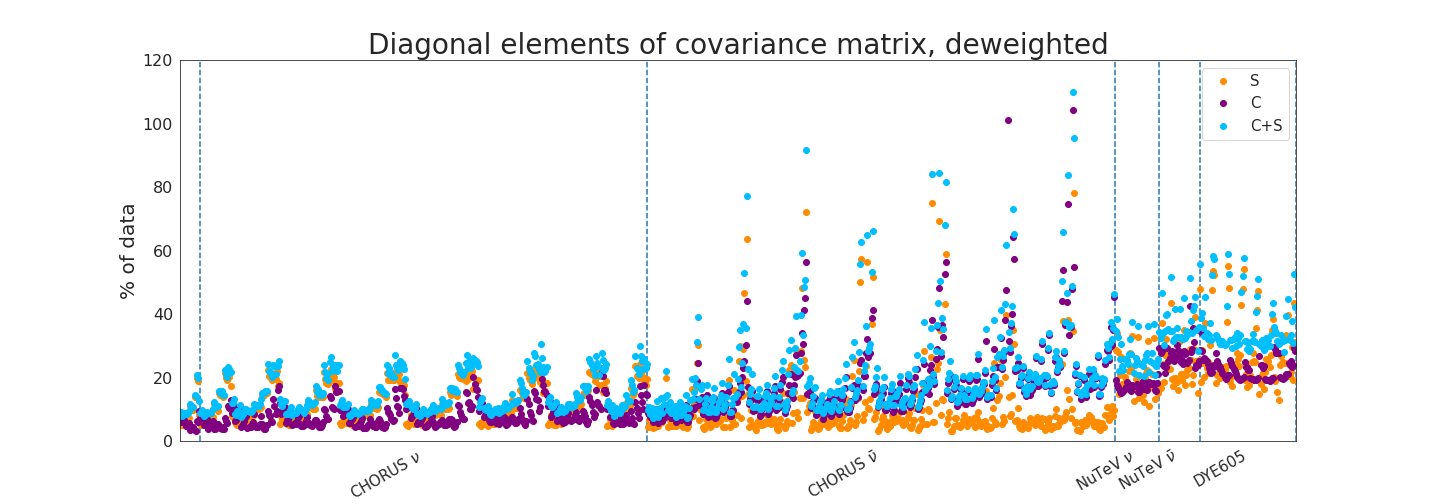
\includegraphics[width=\linewidth, trim={4cm 0 4cm 0}]{nuclear/plots/diag_covmat_deweighted.png}
        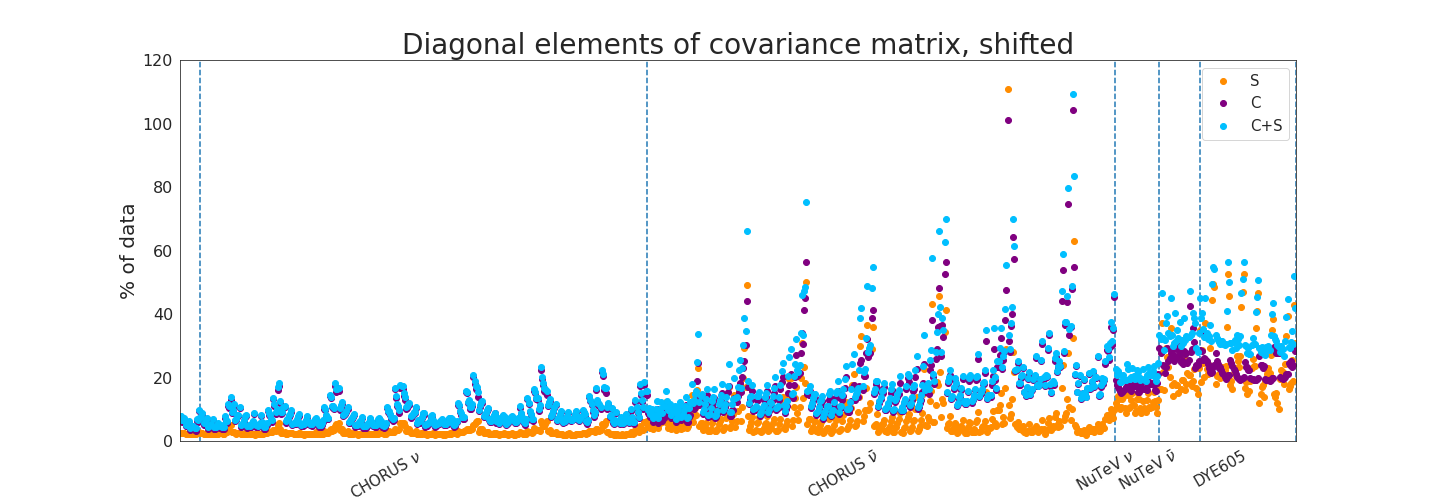
\includegraphics[width=\linewidth, trim={4cm 0 4cm 0}]{nuclear/plots/diag_covmat_shifted.png}
    \caption{Square root of diagonal elements of covariance matrices for $C$ (purple), $S$ (orange) and $C+S$ (blue). All values are displayed as a \% of data. Top: deweighted; bottom:shifted.
    \label{fig:nuccov1} }
    \end{center}
\end{figure}   
%%%%%%%%%%%%%%%%%%%%%%%%%%%%%%%%%%%%%%%%%%%%%%%%%%%%%%%%%%%%%%%%%%%%%
For the deweighted case, it is clear that the heavy nuclear uncertainties are comparable to the experimental uncertainties and are larger in most regions other than CHORUS $\bar{\nu}$. This suggests that all datasets apart from that will be significantly deweighted in the fit. We see that the plot has many features in common with Fig.~\ref{fig:nucobs}, in particular the kinematic pattern, and this makes sense as the covariance matrix is composed using the difference in observables when using nPDFs versus proton ones. For the shifted case, we see a marked decrease in the diagonal of $S$, such that deuteron per-point uncertainties seem no longer significant for CHORUS.
 
 %%%%%%%%%%%%%%%%%%%%%%%%%%%%%%%%%%%%%%%%%%%%%%%%%%%%%%%%%%%%%%%%%%%%%% 
\begin{figure}[h]
  \begin{center} 
    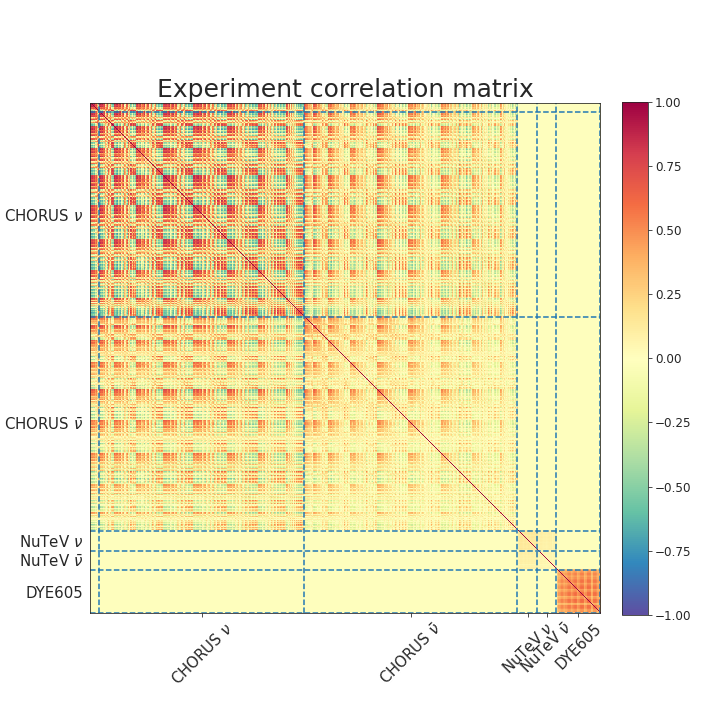
\includegraphics[width=0.45\linewidth]{nuclear/plots/covmats_Experiment_nuclear.png}
    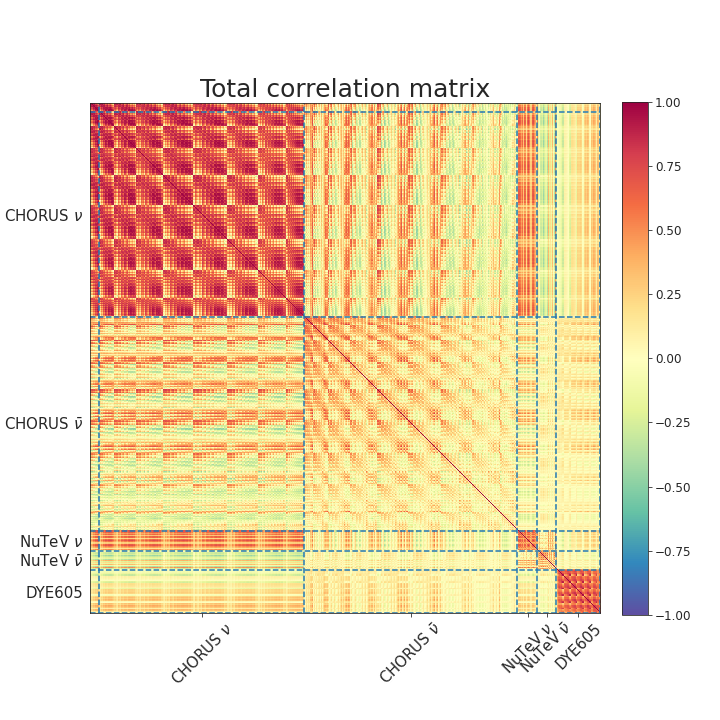
\includegraphics[width=0.45\linewidth]{nuclear/plots/covmats_Total_nuclear.png}
    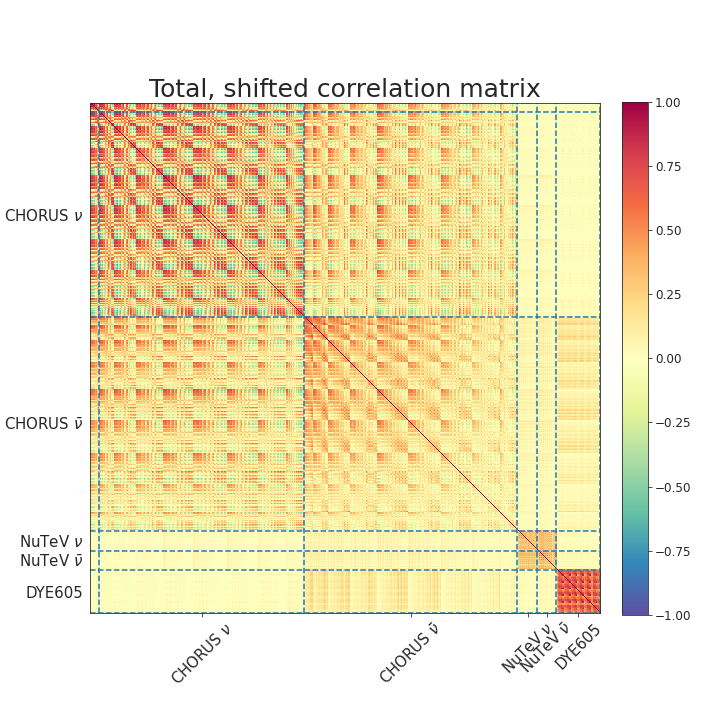
\includegraphics[width=0.45\linewidth]{nuclear/plots/covmats_Total_shifted_nuclear.png}
   \caption{ Correlation matrices for heavy nuclear data. The experiment correlation matrix, $C$, is shown alongside the total correlation matrix, $C+S$, for both the deweighted and the shifted case.
    \label{fig:nuccov} }
  \end{center}
\end{figure}
%%%%%%%%%%%%%%%%%%%%%%%%%%%%%%%%%%%%%%%%%%%%%%%%%%%%%%%%%%%%%%%%%%%%%%

The lower panels of Fig.~\ref{fig:nucobs} investigate the pattern of correlations, displaying correlation matrices as defined in Sec.~\ref{sec:results} of Chapter~\ref{chapter:mhous}. Note that in Ref.~\cite{Ball:2018twp} we considered covariance matrices experiment by experiment (a conservative approach), but here we compute the full heavy nuclear covariance matrix, including correlations between experiments. We display the correlation matrices for both the deweighted and shifted theory covariance matrices. Adding the theory covariance matrix introduces correlations on the off-block diagonals in both cases, but these are particularly strong in the deweighted case. CHORUS $\nu$ shows especially larger correlations upon introducing the deweighted $S$, but these are reduced almost to experiment level when the shifted $S$ is used instead. This is a clear consequence of the systematic shift in Fig.~\ref{fig:nucobs}, which is larger than the uncertainty from the nPDF. Once again, this is evidence that using the shifted formulism is the most appropriate here.

\section{Deuteron uncertainties}
\label{sec:deutunc}
We now turn to uncertainties from deuteron data. The logic is the same as for heavy nuclear uncertainties, except we have a lot more deuteron data than heavy nuclear data from a particular element. This allows us to fit our own deuteron PDFs within the NNPDF methodology, resulting in NNLO PDFs to calculate uncertainties rather than NLO ones. 

The whole procedure is outlined in Fig.~\ref{fig:flowchart}. We split the global data into ``proton" and ``deuteron" data, where the proton data in fact includes the heavy nuclear data considered in the previous section; this allows us to focus purely on deuteron uncertainties. The deuteron data are a combination of ``pure" deuteron data, coming from deuteron-only targets (SLAC and BCDMS), and ``mixed" deuteron data, which are ratios so depend also on proton target data (NMC and DYE866/NuSea). We can denote the pure data as $T_i^d[f_d]$ and the mixed data as $T_i^d[f_d, f_p]$, indicating the additional dependence of the latter on the proton PDF.

In normal proton PDF fits any deuteron observable is calculated using the isoscalar PDF, 
\be
\label{eqn:iso}
f_s = \frac{1}{2} (f_p + f_n),
\ee
where $f_n$ is the neutron PDF, obtained under the assumption of isospin invariance (by swapping $u$ and $d$ quarks in $f_p$).
%%%%%%%%%%%%%%%%%%%%%%%%%%%%%%%%%%%%%%%%%%%%%%%%%%%%%%%%%%%%%%%%%%%%%
\begin{figure}[H]
  \begin{center}
    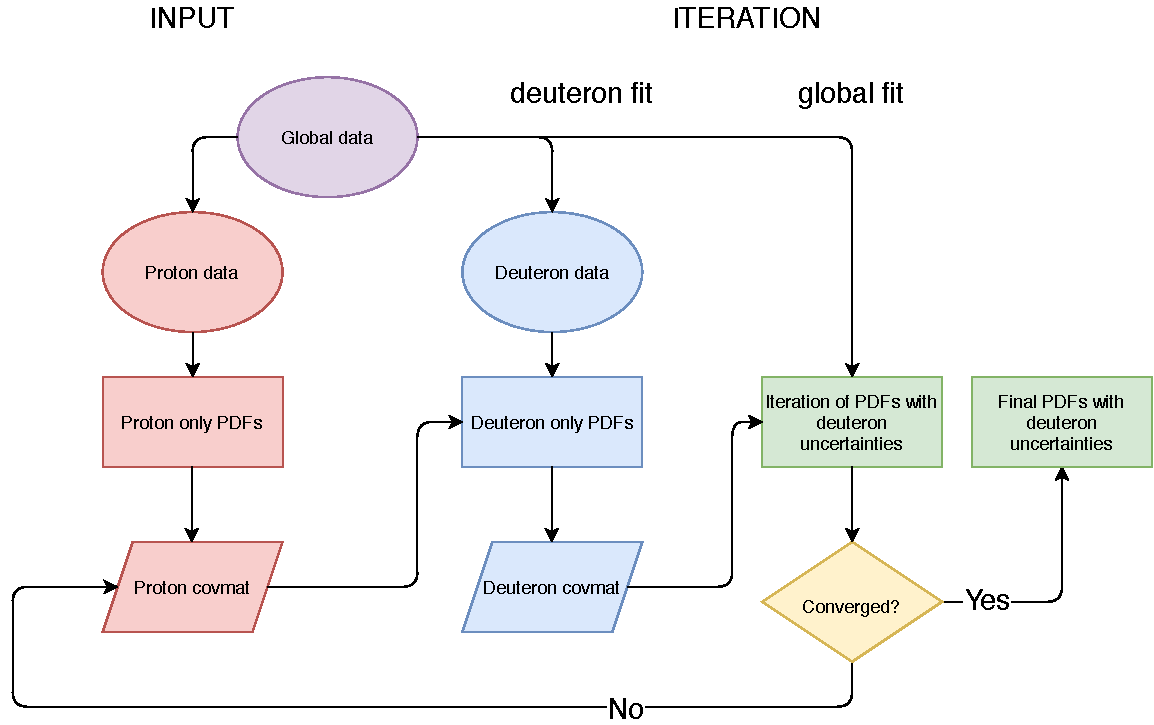
\includegraphics[width=\linewidth]{nuclear/plots/deut_flowchart.pdf}
   \caption{ Outline of the iterative procedure used to determine proton PDFs with deuteron uncertainties. The data is split into proton data and deuteron data. The proton data is used to find proton-only PDFs which are needed to fit deuteron observables in deuteron-only PDFs. These are used to construct a deuteron covariance matrix which is used in a global proton PDF fit. The whole process is iterated to consistency.
    \label{fig:flowchart} }
  \end{center}
\end{figure}
%%%%%%%%%%%%%%%%%%%%%%%%%%%%%%%%%%%%%%%%%%%%%%%%%%%%%%%%%%%%%%%%%%%%%%

The procedure is as follows:
\begin{enumerate}
\item The proton data is used to fit pure proton PDFs (uncontaminated by deuteron data), $\{f_p^{(k)}: k=1,\dots, N_{rep} \}$ with central value $f_p^{0} \equiv f_p$.
\item We cannot fit the pure deuteron PDFs without additional input because of the mixed ratio data ($T_i^d[f_d, f_p]$); these data require a proton PDF as input. We can use $f_p^{0}$ from the proton-only fit here, but since this is only the central value we must include a proton covariance matrix to account for the uncertainty due to the proton PDF. This is composed
\be 
\label{eq:protoncovmatrix}
\begin{split}
&S_{ij}^p = \langle \Delta_i^{p,\ (k)}, \Delta_j^{p,\ (k)} \rangle \\
&\Delta_i^{p,\ (k)} = T_i^d[f_d^{(0)}, f_p^{(k)}] - T_i^d[f_d^{(0)}, f_p^{(0)}],
\end{split}
\ee
where $i$ runs over the deuteron ratio data only. This encapsulates the correlations between the ratio datasets due to their common dependence on the proton PDF.
\item Fit the deuteron PDFs using $C_{ij} + S^p_{ij}$ for the deuteron ratio data. However, in practice $S^p$ depends on $f_d^{(0)}$ and we don't know this yet (that's what we're trying to find!). To first approximation we can replace $f_d^{(0)} \to f_s^{(0)}$, using the isoscalar PDF from Eqn.~\ref{eqn:iso}. This is a reasonable exchange, given that $S_{ij}^p$ is a measure of uncertainty, and acts only to deweight data in the fit; using $f_s$ should have only a very small effect. In principle, we could then iterate this to consistency, using the output $f_d$ to determine a new $S_{ij}^p$ and perform a new deuteron fit. However we are less interested in determining the deuteron PDFs themselves, more in their application in creating a covariance matrix for fitting proton PDFs. Any (already small) effect from using $f_s$ in $S^p$ will become smaller when finding $f_d$ and then smaller again when finding $f_p$, where the only influence is via a covariance matrix which depends on $f_d$.
\item Use $f_d$ to generate a deuteron covariance matrix:
\be 
\label{eq:deuteroncovmatrix}
\begin{split}
&S_{ij}^d = \langle \Delta_i^{d,\ (k)}, \Delta_j^{d,\ (k)} \rangle \\
&\Delta_i^{d,\ (k)} = 
\begin{cases}
T_i^d[f_d^{(k)}] - T_i^d[f_s^{(0)}]  &i \in \text{pure} \\
T_i^d[f_d^{(k)}, f_p^{(0)}] - T_i^d[f_s^{(0)}, f_p^{(0)}] &i \in \text{mixed},
\end{cases}
\end{split}
\ee 
or, for the shifted case,
\be 
\label{eq:deuteronshifted}
\begin{split}
\Delta_i^{d,\ (k)} = 
\begin{cases}
T_i^d[f_d^{(k)}] - T_i^d[f_d^{(0)}]  &i \in \text{pure} \\
T_i^d[f_d^{(k)}, f_p^{(0)}] - T_i^d[f_d^{(0)}, f_p^{(0)}] &i \in \text{mixed}, \\
\end{cases}
\end{split}
\ee
\be
\begin{split}
\delta T_i^d = 
\begin{cases}
T_i^d[f_d^{(0)}] - T_i^d[f_s^{(0)}]  &i \in \text{pure} \\
T_i^d[f_d^{(0)}, f_p^{(0)}] - T_i^d[f_s^{(0)}, f_p^{(0)}] &i \in \text{mixed}.
\end{cases}
\end{split}
\ee
$S^d$ incorporates correlations between the deuteron data due to their common dependence on the deuteron PDF and, for the ratio data, their consequential dependence on poton PDFs.
\item Perform a global proton PDF fit incorporating $S^d$ for the deuteron data. These are PDFS with deuteron uncertainties included.
\item Use the resulting proton PDFs in place of the proton-only PDFs in Step 2, thus iterating the procedure. We expect this to converge rapidly for a few reasons: first, the influence of deuteron data in a proton fit is small; second, a small change in the proton PDF makes little difference to the deuteron uncertainty; third, the effect of deuteron uncertainties on the weight of data in the fit is anticipated to be small.
\end{enumerate}

Note that in this procedure we are not double counting the deuteron data; we use them once to determine the deuteron uncertainty and once to do a global fit to find the proton PDFs. Adding uncertainties actually makes the deuteron data count \textit{less}.

\begin{table}[h]
  \centering
  \scriptsize
  \renewcommand{\arraystretch}{1.13}
  \begin{tabularx}{\textwidth}{lllX}
    \toprule
    {\bf Iteration }  & {\bf Dataset }            & {\bf Fit ID }        & { \bf Description }\\
    \midrule
    Baseline    & Proton and Deuteron & global-base    & NNPDF4.0 fit without nuclear uncertainties\\
    \midrule
    Iteration 0 & Proton              & proton-ite0    & Same as baseline, but restricted to the proton dataset\\
    \midrule
    Iteration 1 & Deuteron            & deuteron-ite1  & Same as baseline, but restricted to the deuteron dataset
                                                         and supplemented with a proton covariance matrix determined
                                                         from the proton-ite0 fit according to
                                                         Eqn.~\ref{eq:protoncovmatrix}.\\
                & Proton and Deuteron & global-ite1-dw & Same as baseline, but supplemented with a deuteron covariance
                                                         matrix determined from the deuteron-ite1 fit according to
                                                         Eqn.~\ref{eq:deuteroncovmatrix}.\\
    \midrule
    Iteration 2 & Deuteron            & deuteron-ite2  & Same as deuteron-ite1, but with a proton covariance matrix
                                                         determined from the global-ite1-dw fit.\\
                & Proton and Deuteron & global-ite2-dw & Same as global-ite1-dw, but with a deuteron covariance matrix
                                                         determined from the deuteron-ite2 fit.\\
                & Proton and Deuteron & global-ite2-sh & Same as global-ite2-sh, but with a deuteron covariance matrix
                                                         and shifts determined according to
                                                         Eqn.~ref{eq:deuteronshifted}.\\
    \bottomrule
  \end{tabularx}
  \caption{A summary of the fits performed in this study, see text for details.}
  \label{tab:fits}
\end{table}


The fits performed are summarised in Tab.~\ref{tab:fits}. The baseline fit, global-base, is equivalent to the base fit in Ref.~\cite{Faura:2020oom}, and is an NNPDF3.1-style fit with minor amendments. We determine a proton-only fit in what we term ``Iteration 0", and then perform two iterations of determining the deuteron and global proton fits, termed ``Iteration 1" and ``Iteration 2". 
%%%%%%%%%%%%%%%%%%%%%%%%%%%%%%%%%%%%%%%%%%%%%%%%%%%%%%%%%%%%%%%%%%%%%
\begin{figure}[h]
  \begin{center}
    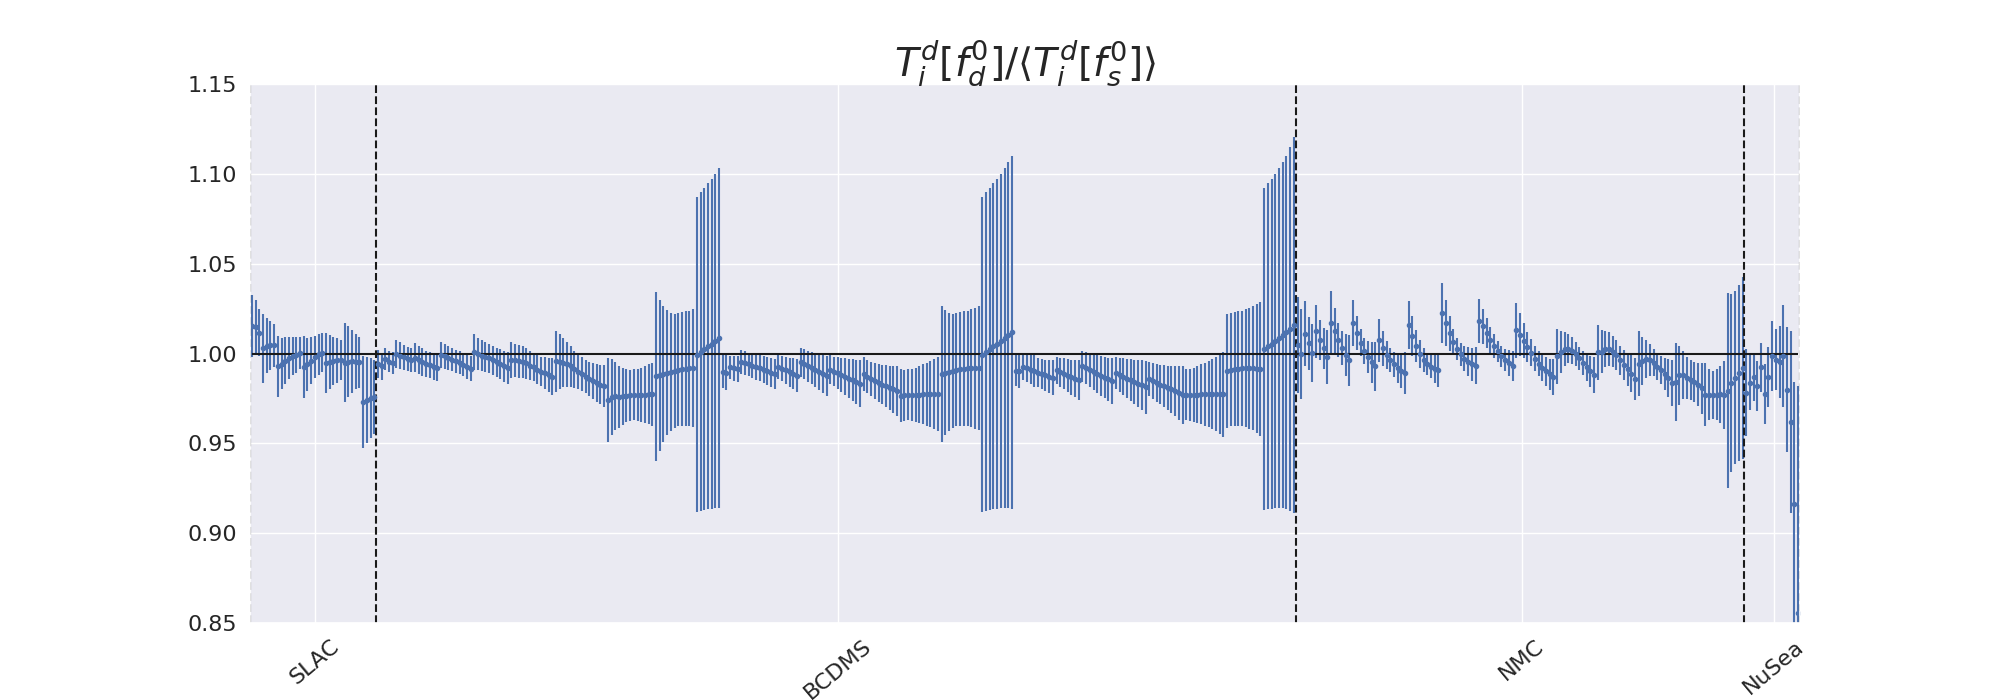
\includegraphics[width=\linewidth, trim={4cm 0 4cm 0}]{nuclear/plots/observable_ratio_ite_1.png}
   \caption{ Like Fig.~\ref{fig:nucobs} but for deuteron observables. Ratio between the deuteron observables computed with Iteration 1 deuteron PDFs, $T_i^d[f_d]$, and the central prediction computed with the isoscalar PDF, $\langle T_i^d[f_s] \rangle$. The error is the standard deviation of the distribution of $T_i^d[f_d]$ replicas. Data are organised in bins of increasing $(x, Q^2)$ within each dataset. 
    \label{fig:deutobs} }
  \end{center}
\end{figure}
%%%%%%%%%%%%%%%%%%%%%%%%%%%%%%%%%%%%%%%%%%%%%%%%%%%%%%%%%%%%%%%%%%%%%%

As in the case for heavy nuclear data, it is useful to first look at the effect on the deuteron observables of using the deuteron PDF rather than the proton one. The uncertainties are quite large but the ratio of observables is consistent with 1 in most regions other than high $(x, Q^2)$, where nuclear shadowing is expected to play a part leading to large negative corrections. This mirrors what was seen in the heavy nuclear case (Fig.~\ref{fig:nucobs}).

\subsection{The deuteron covariance matrix}
We now go on to investigate the deuteron covariance matrix. The diagonal elements are displayed for Iteration 1 in Fig.~\ref{fig:deutcov1}. Again, we see a pattern that parallels the pattern in the deuteron observable ratios; the size of the per-point uncertainty depends on the kinematics. The deuteron uncertainty is smaller than the experimental uncertainty for the  pure deuteron datasets (SLAC and BCDMS), but is comparable for the mixed ratio data (NMC and DYE866/NuSea). This is because ratio data have smaller experimental uncertainties due to a significant cancellation of systematic errors. 

%%%%%%%%%%%%%%%%%%%%%%%%%%%%%%%%%%%%%%%%%%%%%%%%%%%%%%%%%%%%%%%%%%%%%
\begin{figure}[h]
  \begin{center}
      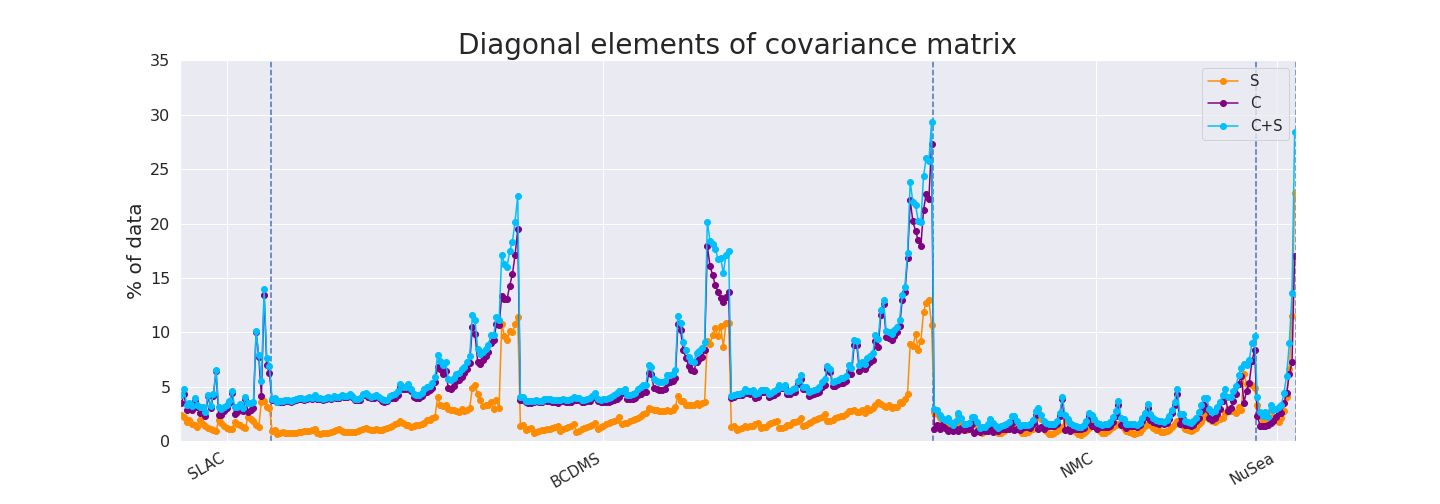
\includegraphics[width=\linewidth, trim={4cm 0 4cm 0}]{nuclear/plots/diag_covmat_ite_1.png}
    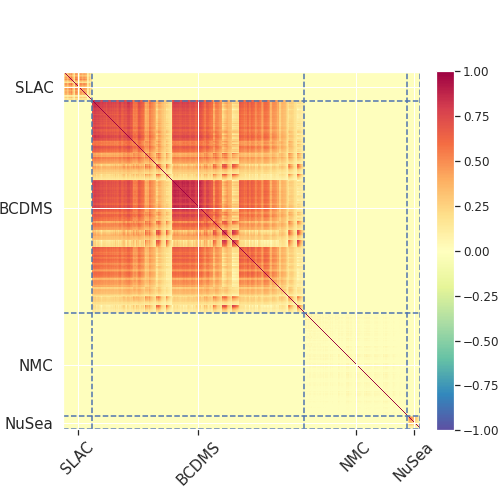
\includegraphics[width=0.45\linewidth]{nuclear/plots/covmats_experiment_global_proton.png}
        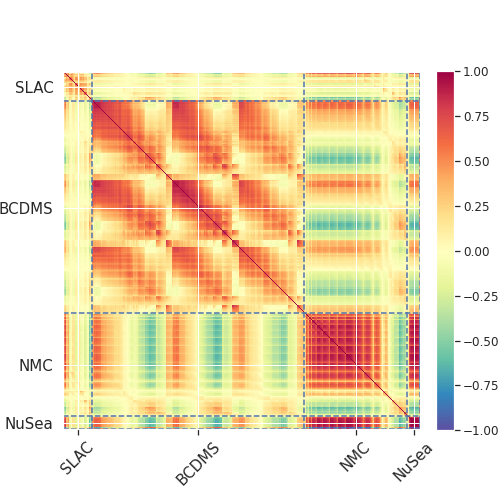
\includegraphics[width=0.45\linewidth]{nuclear/plots/covmats_total_global_proton.png}
    \caption{\textbf{Top panel:} Square root of diagonal elements of covariance matrices for $C$ (purple), $S$ (deweighted; orange) and $C+S$ (deweighted; blue). All values are displayed as a \% of data. \textbf{Bottom panel: }Correlation matrices. $C$ (left) and $C+S$ (deweighted; right). The deweighted case only is displayed, but the qualitative features remain the same for the shifted case.
    \label{fig:deutcov} }
    \end{center}
\end{figure}   
%%%%%%%%%%%%%%%%%%%%%%%%%%%%%%%%%%%%%%%%%%%%%%%%%%%%%%%%%%%%%%%%%%%%%

The bottom part of the figure shows the full matrix plots, and we can see immediately the richness of structure introduced by the deuteron covariance matrix. As above, we see the most impact on the ratio data: NMC and DYE866/NuSea. The figures show only the deweighted case, but this is qualitatively similar to the shifted case. 
\section{PDFs with nuclear corrections}
\label{sec:nucpdfs}
Going to have to use 4.0 PDFs here.
\section{Summary and outlook}
\label{sec:summandoutlook}
